\documentclass[12pt]{article}
\usepackage[margin=2.5cm]{geometry}
\usepackage{natbib} %aas uses natbib


% paragraph spacing
\setlength{\parskip}{.7em}
\setlength{\parindent}{0em}

% maths/symbols
\usepackage{amsmath}
\usepackage{amssymb}

% figures
\usepackage{graphicx}
\graphicspath{{./figures/}}
\usepackage{subcaption} % subfigures

% positioning of figures and tables
\usepackage{float}

% hyperlinks
\usepackage{hyperref}


\title{A Mid-Infrared Analysis of Accreting Supermassive Black Holes}

\author{Mitchell Hooymans (n8869022)}
\date{October 2023}




\begin{document}

\maketitle
\newpage
\tableofcontents
\newpage



\section{Section Title}
This is a template for PVB220 and will be used for PVB304
% This is how you add a comment. This will not appear in the PDF!

    \subsection{References}

    The title is automatically created added to the table of contents. You can also make references 
    \citep{lacy_obscured_2004}

        \subsubsection{Add a table}
        Some import variables we use in cosmology are given in Table \ref{tab:aTable}.
        
            \begin{table}[H]
                \centering
                \caption{A caption}
                \begin{tabular}{lr}
                    \hline \hline
                    Variable & Value  \\
                    \hline 
                    $c$ & $3\times10^{8}$ m/s \\
                    $\gamma$ & Lorentz Factor \\
                    \hline
                \end{tabular}
                \label{tab:aTable}
            \end{table}
            
            
        \subsubsection{Add a figure}
        
        Figures can be added, as shown in Figure \ref{fig:Profiling}.
        
            \begin{figure}[H] % <- This [H] positions the figure here!
                \centering
                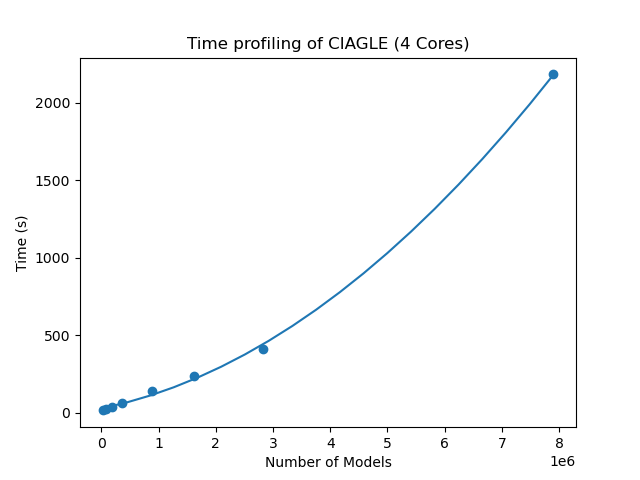
\includegraphics[width=0.7\textwidth]{figures/profiling_time.png}
                \caption{An example figure}
                \label{fig:Profiling}
            \end{figure}
            
    

\newpage
\bibliography{references.bib} % references file!
\bibliographystyle{aasjournal} % referencing style

\appendix


\end{document}